\documentclass[11pt,a4paper]{article}

% Informe corto del Grupo 29: cómo se dividió Santiago en sectores.
% Las cifras vienen de cifras_sectores.tex y el mapa de mapa_sectores.pdf;
% ambos se regeneran con cifras_sectores.py y mapa_sectores.py.

% Estilo común de los informes cortos de esta carpeta.
\usepackage[utf8]{inputenc}
\usepackage[T1]{fontenc}
\usepackage[spanish,es-noshorthands]{babel}
\usepackage{lmodern}
\renewcommand{\familydefault}{\sfdefault}
\usepackage[a4paper,left=2cm,right=2cm,top=2.0cm,bottom=1.5cm]{geometry}
\usepackage[table]{xcolor}
\usepackage{graphicx}
\usepackage{tabularx}
\usepackage{booktabs}
\usepackage{enumitem}
\usepackage[skins]{tcolorbox}
\usepackage{titlesec}
\usepackage{fancyhdr}
\usepackage[font=small,labelfont=bf,skip=4pt]{caption}
\usepackage[hidelinks]{hyperref}

% ---------- Colores (los de sector son los mismos del mapa) ----------
\definecolor{azul}{HTML}{1F4E79}
\definecolor{azulclaro}{HTML}{E8F0F8}
\definecolor{verdeclaro}{HTML}{EAF5EA}
\definecolor{naranjoclaro}{HTML}{FFF3E0}
\definecolor{gris}{HTML}{5F6B76}
\definecolor{sector1}{HTML}{E34948}
\definecolor{sector2}{HTML}{2A78D6}
\definecolor{sector3}{HTML}{1BAF7A}
\definecolor{sector4}{HTML}{EDA100}
\definecolor{sector5}{HTML}{008300}
\newcommand{\cuadro}[1]{\textcolor{#1!82!white}{\rule[-0.5pt]{7pt}{7pt}}\hspace{3pt}}

% ---------- Títulos, encabezado y espacios ----------
\titleformat{\section}{\large\bfseries\color{azul}}{}{0pt}{}
\titlespacing*{\section}{0pt}{0.9em}{0.25em}
\setlength{\headheight}{13pt}
\pagestyle{fancy}
\fancyhf{}
\lhead{\small\color{gris}Grupo 29 · Capstone · Buses eléctricos en Santiago}
\rhead{\small\color{gris}\thepage\ de 2}
\renewcommand{\headrulewidth}{0.4pt}
\setlength{\parindent}{0pt}
\setlength{\parskip}{0.45em}
\setlist{leftmargin=1.4em,itemsep=0.2em,topsep=0.2em,parsep=0pt}
\newtcolorbox{caja}[2][azulclaro]{colback=#1,colframe=#1,boxrule=0pt,arc=2pt,
  left=7pt,right=7pt,top=5pt,bottom=5pt,fonttitle=\bfseries\color{azul},
  coltitle=azul,title={#2},attach title to upper={\par\vspace{2pt}}}


% Archivo generado por cifras_sectores.py. No editar a mano.
\newcommand{\TotalRutas}{417}
\newcommand{\TotalCorridas}{64.502}
\newcommand{\TotalPlazas}{700}
\newcommand{\RutasAjustadas}{110}
\newcommand{\PctRutasAjustadas}{26}
\newcommand{\RutaEjemplo}{101}
\newcommand{\NombreRutaEjemplo}{Recoleta--Cerrillos}
\newcommand{\GanadorEjemplo}{El Conquistador}
\newcommand{\FilasSectores}{%
\cuadro{sector1} 1 & Vespucio Norte & 65 & 8.744 & 14\,\% \\
\cuadro{sector2} 2 & El Conquistador & 95 & 14.258 & 22\,\% \\
\cuadro{sector3} 3 & Los Espinos & 68 & 11.027 & 17\,\% \\
\cuadro{sector4} 4 & La Reina & 72 & 11.486 & 18\,\% \\
\cuadro{sector5} 5 & Santa Rosa & 117 & 18.987 & 29\,\% \\%
}
\newcommand{\FilasEjemplo}{%
Vespucio Norte & 54,0 \\
\rowcolor{azulclaro}\textbf{El Conquistador} & \textbf{44,6} \\
Los Espinos & 49,7 \\
La Reina & 72,5 \\
Santa Rosa & 51,6 \\%
}


\begin{document}

{\LARGE\bfseries\color{azul} ¿Cómo dividimos Santiago en cinco sectores?}\par
\vspace{2pt}
{\large\color{gris} La idea, explicada sin fórmulas}\par
\vspace{6pt}

\begin{caja}{En una frase}
Repartimos las \TotalRutas{} rutas de buses de Santiago en cinco grupos, uno por cada lugar donde
los buses eléctricos pueden cargar. Cada ruta queda en el grupo del lugar de carga que le queda más a mano.
A cada grupo lo llamamos \textbf{sector}.
\end{caja}

\section{1. ¿Qué queremos resolver?}
En un día laboral, los buses de Santiago hacen \TotalCorridas{} \textbf{corridas}. Una corrida es un viaje
de un bus de punta a punta de su ruta. Nuestro trabajo es decidir qué bus eléctrico hace cada corrida, y
cuándo y dónde carga su batería, usando la menor cantidad posible de buses y gastando lo menos posible.

Los buses solo pueden cargar en cinco lugares, llamados \textbf{electroterminales}: Vespucio Norte,
El Conquistador, Los Espinos, La Reina y Santa Rosa. Entre los cinco tienen \TotalPlazas{} puestos para buses.

\section{2. ¿Por qué dividir la ciudad?}
Si cualquier bus pudiera hacer cualquier corrida de la ciudad, habría tantas combinaciones posibles que el
problema sería demasiado grande para resolverlo de una sola vez. Además, casi nunca conviene mandar un bus de
Quilicura a hacer un viaje en Puente Alto: todo lo que maneja sin pasajeros gasta batería y tiempo.

Por eso, antes de optimizar, ordenamos la ciudad. Cada bus trabaja con un grupo de rutas que están cerca
unas de otras y cerca de un mismo electroterminal.

\section{3. ¿Cómo se decide el sector de una ruta?}
\begin{minipage}[t]{0.585\linewidth}
La regla tiene tres pasos y es la misma para todas las rutas:
\begin{enumerate}
  \item \textbf{Miramos los extremos.} Anotamos dónde parte y dónde termina la ruta, en sus dos sentidos.
  \item \textbf{Medimos el camino a cada electroterminal.} Para cada uno de los cinco, calculamos cuántos
        kilómetros manejaría un bus sin pasajeros: desde el electroterminal hasta donde parte la ruta, y
        desde donde termina de vuelta al electroterminal. Se mide por las calles y respetando el sentido
        del tránsito, no en línea recta.
  \item \textbf{Elegimos la suma más baja.} Sumamos esos kilómetros y la ruta queda en el sector del
        electroterminal que suma menos.
\end{enumerate}
Es como asignar a cada niño al colegio que le queda más cerca caminando por las calles, y no al que se ve
más cerca en el mapa.
\end{minipage}\hfill
\begin{minipage}[t]{0.385\linewidth}
\vspace{0pt}
\begin{caja}{Ejemplo: la ruta \RutaEjemplo\\{\normalfont\small\color{gris}\NombreRutaEjemplo}}
\small
\begin{tabularx}{\linewidth}{@{}Xr@{}}
\toprule
Electroterminal & km sin pasajeros \\
\midrule
\FilasEjemplo
\bottomrule
\end{tabularx}

\vspace{3pt}
La suma más baja es la de \GanadorEjemplo{}. La ruta \RutaEjemplo{} queda en ese sector.
\end{caja}
\end{minipage}

\section{4. Tres reglas que ordenan todo}
\begin{itemize}
  \item \textbf{Una ruta, un sector.} La ida y la vuelta de una ruta, y todas sus variantes, quedan siempre juntas.
  \item \textbf{Un bus, un sector.} Durante el día, un bus solo hace corridas de rutas de su sector. Dentro
        del sector sí puede pasar de una ruta a otra, y así se aprovecha mejor cada bus.
  \item \textbf{Los cargadores son de todos.} El sector lleva el nombre de un electroterminal, pero eso no
        obliga a cargar ahí. Un bus puede cargar en cualquiera de los cinco. El modelo revisa que ninguno
        reciba más buses de los que le caben.
\end{itemize}
Los sectores son los mismos para el día laboral, el sábado y el domingo.

\newpage

\begin{figure}[t]
\centering
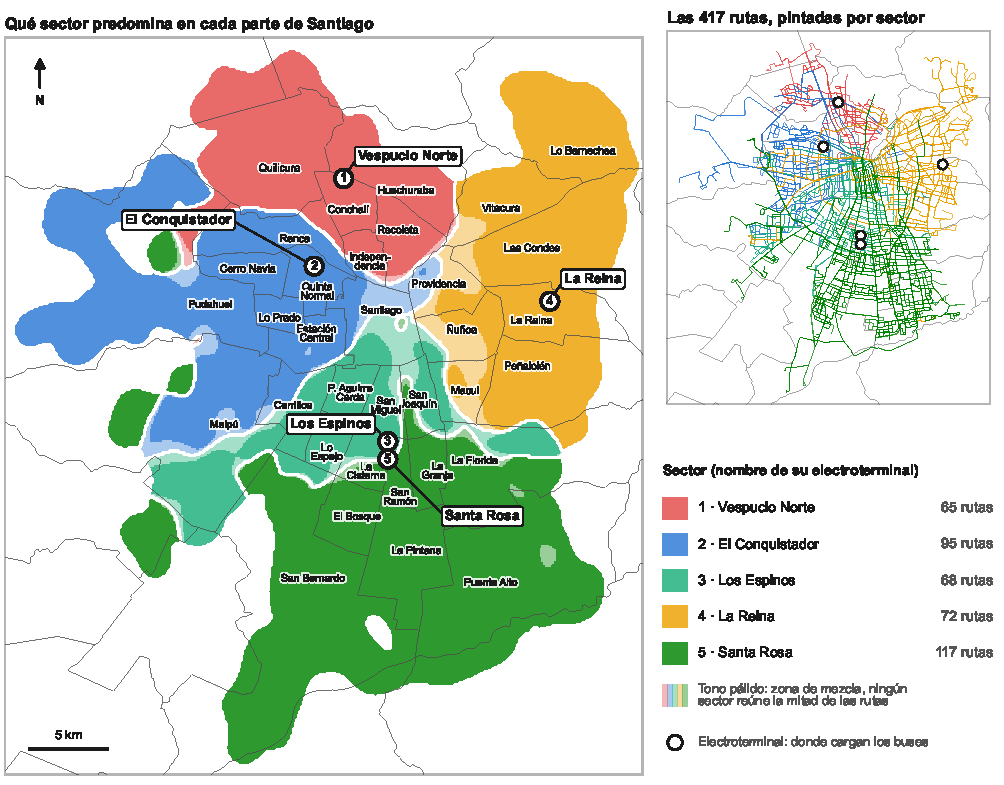
\includegraphics[width=\linewidth]{mapa_sectores.pdf}
\caption*{\textbf{El mapa de los sectores.} A la izquierda, cada parte de Santiago tiene el color del sector al
que pertenece la mayoría de las rutas que pasan por ahí. A la derecha están las rutas reales. Los nombres en
letra chica son comunas.}
\end{figure}

\section{5. Cómo leer el mapa}
\begin{itemize}
  \item \textbf{Un sector es un grupo de rutas, no un territorio.} Los colores son una ayuda para verlo.
        Las rutas reales cruzan esas fronteras.
  \item \textbf{En el centro se mezclan todos.} Ahí pasan rutas de los cinco sectores, y por eso el color es más pálido.
  \item \textbf{Las manchas sueltas son rutas largas.} Las verdes del poniente son rutas del sector
        Santa Rosa.
  \item \textbf{El sur tiene dos sectores.} Los Espinos y Santa Rosa están a cerca de un kilómetro y se
        reparten el sur.
\end{itemize}

\vspace{2pt}
\begin{minipage}[t]{0.50\linewidth}
\vspace{0pt}
{\bfseries\color{azul} Tamaño de cada sector en un día laboral}\par\vspace{3pt}
\small
\begin{tabularx}{\linewidth}{@{}lXrrr@{}}
\toprule
Sector & Electroterminal & Rutas & Corridas & \% \\
\midrule
\FilasSectores
\midrule
 & \textbf{Total} & \textbf{\TotalRutas} & \textbf{\TotalCorridas} & \textbf{100\,\%} \\
\bottomrule
\end{tabularx}
\end{minipage}\hfill
\begin{minipage}[t]{0.47\linewidth}
\vspace{0pt}
\begin{caja}[verdeclaro]{Qué ganamos}
\small
El problema se vuelve manejable. Cada bus trabaja cerca de donde ya está. La regla es simple y
depende solo de distancias.
\end{caja}
\vspace{1pt}
\begin{caja}[naranjoclaro]{Qué cedemos}
\small
No probamos combinaciones entre sectores, y ahí puede quedar ahorro sin aprovechar. En \RutasAjustadas{}
rutas (\PctRutasAjustadas\,\%) el segundo electroterminal queda a menos de 5\,\% del primero. La regla
no mira horarios ni cuántos buses caben en cada electroterminal.
\end{caja}
\end{minipage}

\end{document}
